%!TEX root = ../egpaper_for_review.tex

\tikzstyle{nS}=[circle,minimum size = 0.6cm,inner sep = 0pt,draw, font=\small,align=left]
\tikzstyle{eS}=[thick,minimum size = 0.5cm,inner sep = 0pt,draw, font=\small,align=left]
\tikzstyle{eC}=[very thick,minimum size = 0.5cm,inner sep = 0pt,draw=red, font=\small,align=left]
\tikzstyle{eNC}=[very thick,minimum size = 0.5cm,inner sep = 0pt,draw=green, font=\small,align=left]
\tikzstyle{eNS}=[fill=white,minimum size = 0.5cm,inner sep = 0pt, font=\tiny,align=left]

\begin{center}
\begin{figure*}
\resizebox{!}{0.15\linewidth}{%
    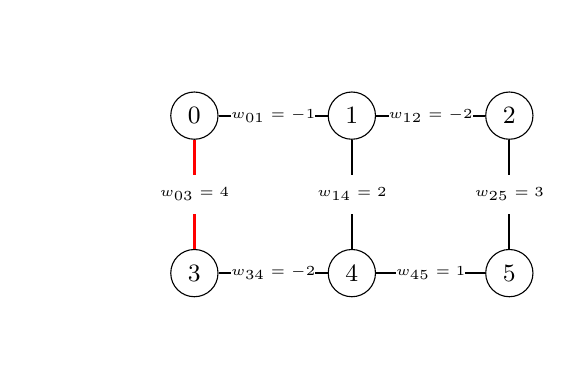
\begin{tikzpicture}
    \draw (0,-1)node (dummyLow){} ;
    \draw (0, 3)node (dummyLow){} ;
    \draw (2,2) node[nS] (n0) {$0$}; 
    \draw (4,2) node[nS] (n1) {$1$};
    \draw (6,2) node[nS] (n2) {$2$};
    \draw (2,0) node[nS] (n3) {$3$}; 
    \draw (4,0) node[nS] (n4) {$4$};
    \draw (6,0) node[nS] (n5) {$5$};


    \path
        (n0) edge[eS] node[eNS]{$w_{01}=-1$} (n1) 
        (n1) edge[eS] node[eNS]{$w_{12}=-2$} (n2) 
        (n3) edge[eS] node[eNS]{$w_{34}=-2$} (n4) 
        (n4) edge[eS] node[eNS]{$w_{45}=1$} (n5)
        (n0) edge[eC] node[eNS]{$w_{03}=4$} (n3)
        (n1) edge[eS] node[eNS]{$w_{14}=2$} (n4)
        (n2) edge[eS] node[eNS]{$w_{25}=3$} (n5)
    ;
    \end{tikzpicture}
    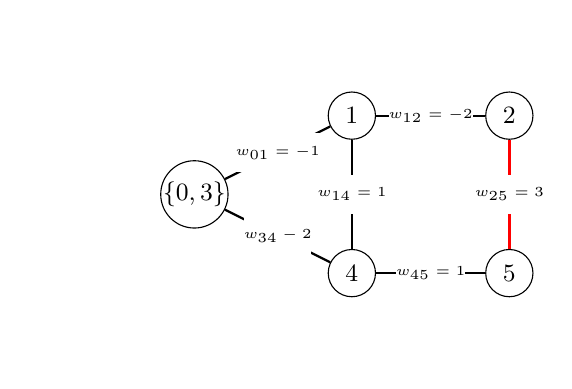
\begin{tikzpicture}
    \draw (0,-1)node (dummyLow){} ;
    \draw (0, 3)node (dummyLow){} ;
    \draw (2,1) node[nS] (n03) {$\{0,3\}$}; 
    \draw (4,2) node[nS] (n1) {$1$};
    \draw (6,2) node[nS] (n2) {$2$};
    \draw (4,0) node[nS] (n4) {$4$};
    \draw (6,0) node[nS] (n5) {$5$};


    \path
        (n03) edge[eS] node[eNS]{$w_{01}=-1$} (n1) 
        (n1) edge[eS] node[eNS]{$w_{12}=-2$} (n2) 
        (n03) edge[eS] node[eNS]{$w_{34}-2$} (n4) 
        (n4) edge[eS] node[eNS]{$w_{45}=1$} (n5)
        (n1) edge[eS] node[eNS]{$w_{14}=1$} (n4)
        (n2) edge[eC] node[eNS]{$w_{25}=3$} (n5)
    ;
    \end{tikzpicture}
}
%
\resizebox{!}{0.15\linewidth}{%
    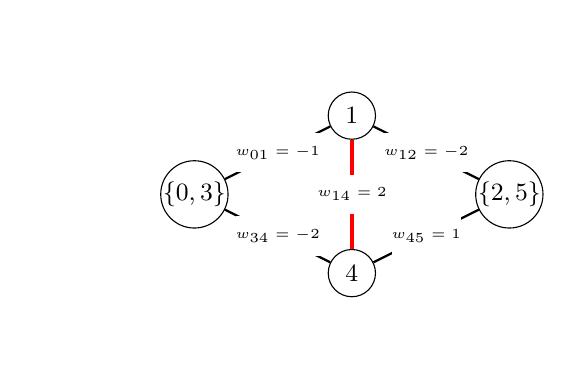
\begin{tikzpicture}
    \draw (0,-1)node (dummyLow){} ;
    \draw (0, 3)node (dummyLow){} ;
    \draw (2,1) node[nS] (n03) {$\{0,3\}$}; 
    \draw (4,2) node[nS] (n1) {$1$};
    \draw (6,1) node[nS] (n25) {$\{2,5\}$};
    \draw (4,0) node[nS] (n4) {$4$};
    \path
        (n03) edge[eS] node[eNS]{$w_{01}=-1$} (n1) 
        (n1) edge[eS] node[eNS]{$w_{12}=-2$} (n25) 
        (n03) edge[eS] node[eNS]{$w_{34}=-2$} (n4) 
        (n4) edge[eS] node[eNS]{$w_{45}=1$} (n25)
        (n1) edge[eC] node[eNS]{$w_{14}=2$} (n4)
    ;
    \end{tikzpicture}
    \begin{tikzpicture}
    \draw (0,-1)node (dummyLow){} ;
    \draw (0, 3)node (dummyLow){} ;
    \draw (2,1) node[nS] (n03) {$\{0,3\}$}; 
    \draw (4,1) node[nS] (n14) {$\{1,4\}$};
    \draw (6,1) node[nS] (n25) {$\{2,5\}$};
    \path
        %(n03) edge[eS] node[eNS]{$w_{01}$} (n1) 
        (n14) edge[eNC] node[eNS]{$w_{12}+$\\$w_{45}=$\\$-1$} (n25) 
        (n03) edge[eS] node[eNS]{$w_{01}+$\\$w_{34}=$\\$-3$} (n14) 
    ;
    \end{tikzpicture}
}
\caption{
    To use hierarchical clustering as an approximator for
    the multicut objective we contract the edge with the highest weight
    in each step (to be contracted edge is shown in red). 
    Whenever multiple edges are merged into a single edge,
    we use the sum of the weight as a new weight, since
    we have to pay for all edges which are cut in the uncontracted 
    graph.
    We stop when the highest edge weight is smaller
    or equal to zero (edge shown in green).
}\label{fig:hc_alg}
\end{figure*}
\end{center}



